\section{Usage and limitation}
We test the Transfer System with 100 million $J/\psi$ data 
which takes about 5TB disk space. It took 5 days to transfer 
these data from IHEP to JINR. The throughput is show in 
figure \ref{fig:throughput}.

\begin{figure}[htbp]
    \begin{center}
        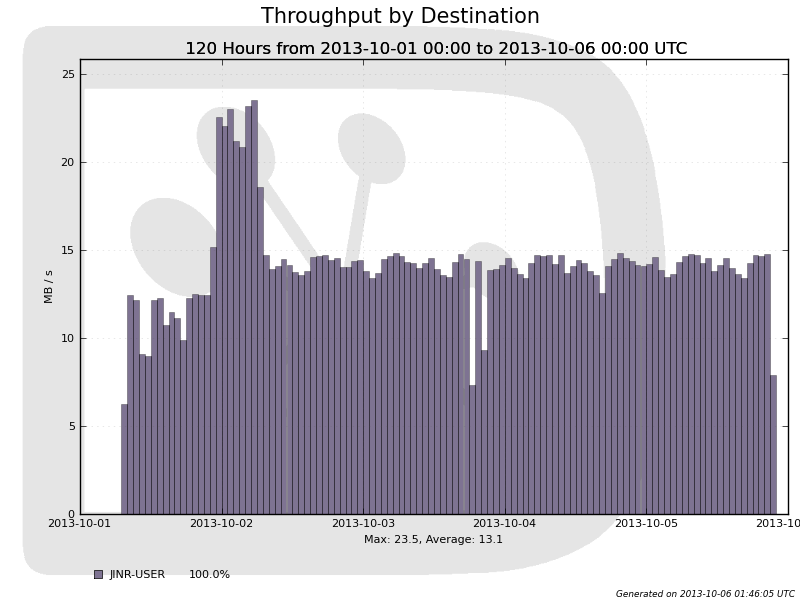
\includegraphics[width=.8\textwidth, keepaspectratio]{data/throughput-dest-1001-10-06.png}
    \end{center}
    \caption{\label{fig:throughput}Throughput from Oct.1 to Oct.6}
\end{figure}

The BESDIRAC Transfer System is not so robust
because of lacking of the experience of DIRAC developing.
When the dataset is small, we don't find any problems.
But when the dataset became huge, some unexpected errors occurred.
\begin{itemize}
    \item The proxy certificates of the users became expired
            because of the long time waiting.
    \item Some files' status always show ``transfer''.
            But in fact the process had already terminated.
    \item All the transfer processes are in the DIRAC server,
            It may occupy too many resources in the server.
\end{itemize}
